% PÔSTER CIENTÍFICO - XXIX ENMC / XVII ECTM 2026
% Inteligência Artificial Aplicada à Detecção de Caprinos em Ambiente Confinado
% ============================================================================
% Codificação: UTF-8
% Classe: a0poster (tamanho A0, orientação retrato)
%
\documentclass[a0,portrait]{a0poster}

% Pacotes essenciais
\usepackage[utf8]{inputenc}
\usepackage[T1]{fontenc}
\usepackage{graphicx}
\usepackage{multicol}
\usepackage{xcolor}
\usepackage{geometry}
\usepackage{fancyhdr}
\usepackage{array}
\usepackage{colortbl}
\usepackage{amsmath}
\usepackage{wrapfig}
\usepackage{caption}
\usepackage{subcaption}
\usepackage{helvet}
\renewcommand{\familydefault}{\sfdefault}
\usepackage{tikz}

% Configurações de cores
\definecolor{darkblue}{RGB}{0, 51, 102}
\definecolor{lightgray}{RGB}{240, 240, 240}
\definecolor{darkgray}{RGB}{80, 80, 80}

% Configurações de layout
\geometry{
    margin=2cm,
    top=2.5cm,
    bottom=2.5cm,
    left=2.5cm,
    right=2.5cm
}

\setlength{\parindent}{0pt}
\setlength{\parskip}{0.5cm}

% Estilos de fontes
\newcommand{\titlefont}{\fontsize{80}{96}\selectfont\bfseries}
\newcommand{\authorsfont}{\fontsize{38}{50}\selectfont\bfseries}
\newcommand{\affiliationfont}{\fontsize{34}{46}\selectfont\itshape}
\newcommand{\sectionfont}{\fontsize{34}{46}\selectfont\bfseries}
\newcommand{\bodyfont}{\fontsize{25}{31}\selectfont}

% Definir cabeçalho do pôster
\setlength{\columnsep}{2cm}
\pagestyle{empty}

\begin{document}

% ============================================================================
% BANNER DO EVENTO (CABEÇALHO)
% ============================================================================
\begin{center}
    
\includegraphics[width=0.9\textwidth]{figures/logo.png}
\end{center}

\vspace{1.5cm}
% ============================================================================
% TÍTULO, AUTORES E AFILIAÇÕES
% ============================================================================
\begin{center}
    % Título principal
    {\titlefont INTELIGÊNCIA ARTIFICIAL APLICADA À DETECÇÃO DE CAPRINOS EM AMBIENTE CONFINADO}

    \vspace{0.6cm}

    % Autores
    {\authorsfont Vinícius Latini Gonçalves\textsuperscript{1}, Gabriel Vaz Bernardini Ferreira\textsuperscript{2}, Felipe Girardi Siqueira\textsuperscript{2}, \\Luciana Conceição D. Campos\textsuperscript{1}, Érica da Costa Reis Carvalho\textsuperscript{2}, Acir Moreno Soares Júnior\textsuperscript{2}}

    \vspace{0.3cm}

    % Afiliações
    {\affiliationfont
    \textsuperscript{1}Universidade Federal de Juiz de Fora (UFJF) - Juiz de Fora - MG\\
    \textsuperscript{2}Universidade Federal de São João del-Rei (UFSJ) - São João del-Rei - MG
    }

    \vspace{1cm}
\end{center}

\vspace{0.5cm}

% ============================================================================
% CORPO DO PÔSTER
% ============================================================================
\begin{multicols}{2}

% ============================================================================
% INTRODUÇÃO
% ============================================================================
{\sectionfont INTRODUÇÃO}

{\bodyfont
O uso de Visão Computacional vem se expandindo na zootecnia de precisão, viabilizando o monitoramento automatizado de animais em confinamento. Contudo, a aplicação de detectores genéricos em condições reais ainda esbarra em variações severas de \textbf{perspectiva de captura} (frontal ou superior) e \textbf{iluminação} (diurna ou noturna/infravermelho).

Este trabalho propõe uma arquitetura de \textbf{Mistura de Especialistas} (\textit{Mixture of Experts} -- MoE) para a detecção, com classe única \texttt{goat}, de caprinos da raça \textit{Saanen} em ambiente de confinamento na UFSJ. Uma rede de roteamento (\textit{gating network}) baseada em \textit{EfficientNet} classifica exclusivamente o \textbf{cenário de captura} -- e não o animal -- direcionando cada vídeo a um dentre quatro detectores YOLOv8 especializados por combinação de perspectiva e iluminação.
}

\vspace{1cm}

% ============================================================================
% METODOLOGIA
% ============================================================================
{\sectionfont METODOLOGIA}

{\bodyfont
\textbf{Dataset:} vídeos capturados por 4 câmeras fixas (\texttt{Cam01}--\texttt{Cam04}), $1280\times960$ px a 8 FPS, ao longo de 36 sessões de gravação (7 dias, rebanho fixo de 8 indivíduos). Rotulação manual (classe única \texttt{goat}) com a ferramenta \textit{EasyLabel}, desenvolvida por alunos da UFSJ.
}

\begin{center}
\begin{tabular}{|l|c|c|c|}
\hline
\textbf{Cenário} & \textbf{Imagens} & \textbf{Caixas} & \textbf{Sessões} \\
\hline
Frente Dia & 2.022 & 16.185 & 8 \\
Frente Noite & 2.001 & 16.008 & 13 \\
Cima Dia & 2.549 & 18.258 & 6 \\
Cima Noite & 2.032 & 16.254 & 9 \\
\hline
\textbf{Total} & \textbf{8.604} & \textbf{66.705} & \textbf{36} \\
\hline
\end{tabular}
\\{\footnotesize\centering Tabela 1 -- Caracterização do dataset por cenário operacional\par}
\end{center}

{\bodyfont
\textbf{Validação -- Temporal K-Fold ($K=5$):} imagens quase-idênticas de vídeo contínuo (8 FPS) causariam vazamento de dados (\textit{leakage}) em um K-Fold aleatório convencional. Adotou-se um particionamento por \textbf{blocos temporais contíguos} dentro de cada sessão, com \textbf{purge buffer de 15 quadros} nas bordas treino/validação, eliminando quase-duplicatas na fronteira. Auditoria confirmou $0\%$ de sobreposição exata entre treino e validação em todos os \textit{folds}.

\textbf{Modelo base:} YOLOv8m, entrada $640\times640$ px, até 300 épocas, \textit{batch size} automático, \textit{early stopping} (\textit{patience}=30).
}

\vspace{0.8cm}

\begin{center}
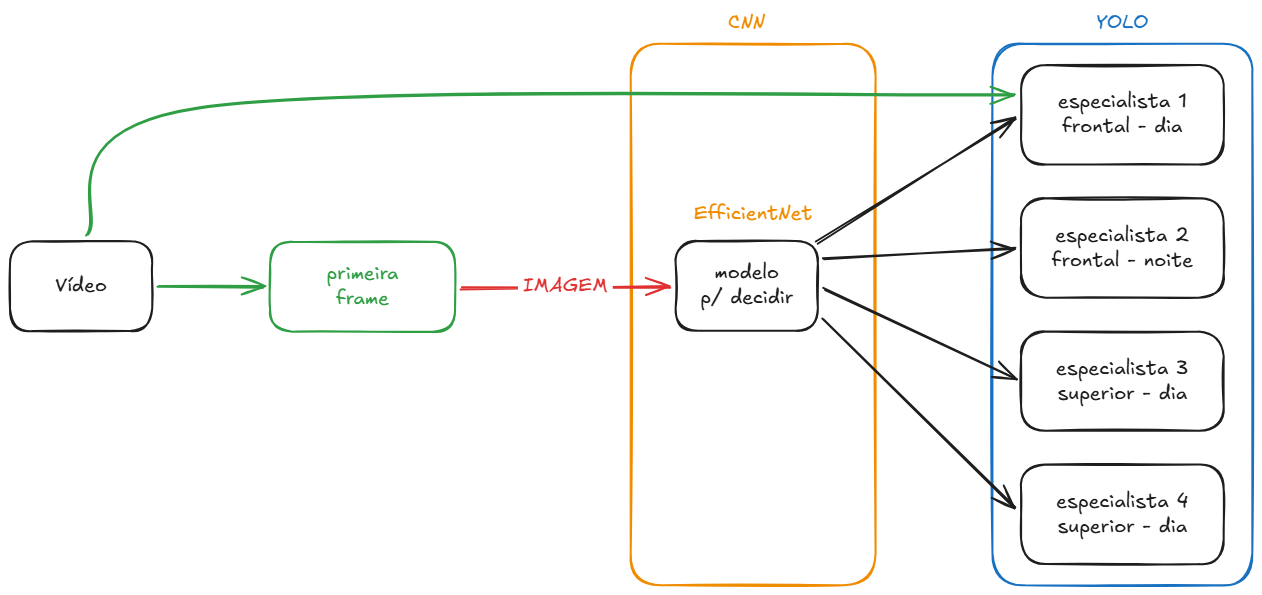
\includegraphics[width=0.95\columnwidth]{figures/moe.png}
\\{\bodyfont Figura 1 -- Arquitetura MoE: roteamento por cenário + 4 especialistas YOLOv8}
\end{center}

\vspace{1cm}

% ============================================================================
% RESULTADOS
% ============================================================================
{\sectionfont RESULTADOS}

{\bodyfont
\textbf{Rede de roteamento (\textit{gating network}):} convergência em 9 épocas, Precisão/Revocação/\textit{F1-Score} $=1{,}00$ em 272 imagens de teste. Análise de \textit{Occlusion} mostrou que padrões do ambiente (parede, cercado) são determinantes para a classificação do cenário, robusta a variações de iluminação.

\textbf{Especialistas YOLOv8 (melhor \textit{fold}):} desempenho elevado e consistente nos 4 cenários, com $mAP_{50}$ saturado em $0{,}9950$.
}

\begin{center}
\begin{tabular}{|l|c|c|c|}
\hline
\textbf{Modelo} & \textbf{F1} & \textbf{mAP50} & \textbf{mAP50-95} \\
\hline
Frontal Dia & 0,9971 & 0,9950 & 0,9015 \\
Frontal Noite & 0,9970 & 0,9950 & 0,8821 \\
Superior Dia & 0,9997 & 0,9950 & 0,8645 \\
Superior Noite & 0,9975 & 0,9950 & 0,8338 \\
\hline
\textbf{Baseline (Overall)} & \textbf{0,9953} & \textbf{0,9948} & \textbf{0,8773} \\
\hline
\end{tabular}
\\{\footnotesize\centering Tabela 2 -- Especialistas MoE vs. baseline monolítico (YOLOv8m único, dataset unificado, mesmo protocolo K-Fold)\par}
\end{center}

{\bodyfont
Nas métricas agregadas, o baseline monolítico (YOLOv8m treinado na união dos 4 cenários) iguala-se aos especialistas -- o ganho da MoE \textbf{não está no mAP bruto}, e sim em: \textbf{(i) modularidade} (novo cenário = novo especialista, sem retreinar o todo); \textbf{(ii) isolamento de falhas} por cenário; \textbf{(iii) explicabilidade} do roteamento via \textit{Occlusion}.

\textbf{Evidência qualitativa (contagem de caixas em inferência, 4 vídeos-teste, 80 quadros, 8 indivíduos/quadro = 640 esperadas):}
}

\begin{center}
\begin{tabular}{|l|c|c|c|}
\hline
\textbf{Cenário} & \textbf{Overall} & \textbf{MoE} & \textbf{Esperado} \\
\hline
Frente Dia & 623 & \textbf{640} & 640 \\
Frente Noite & 643 & \textbf{640} & 640 \\
Cima Dia & 532 & \textbf{640} & 640 \\
Cima Noite & 663 & \textbf{640} & 640 \\
\hline
\end{tabular}
\\{\footnotesize\centering Tabela 3 -- MoE acerta 100\% da contagem esperada nos 4 vídeos; baseline sub/sobredetecta\par}
\end{center}

{\bodyfont
O baseline monolítico subdetecta em \textit{Cima Dia} (oclusão entre indivíduos agrupados) e sobredetecta em \textit{Cima/Frente Noite} (caixas duplicadas com $IoU=0{,}64$, abaixo do limiar de NMS). O especialista MoE correspondente acerta as 640 caixas em todos os 4 cenários, com confiança média de $0{,}91$ (variação $0{,}74$--$0{,}96$).
}

\vspace{0.8cm}

\begin{center}
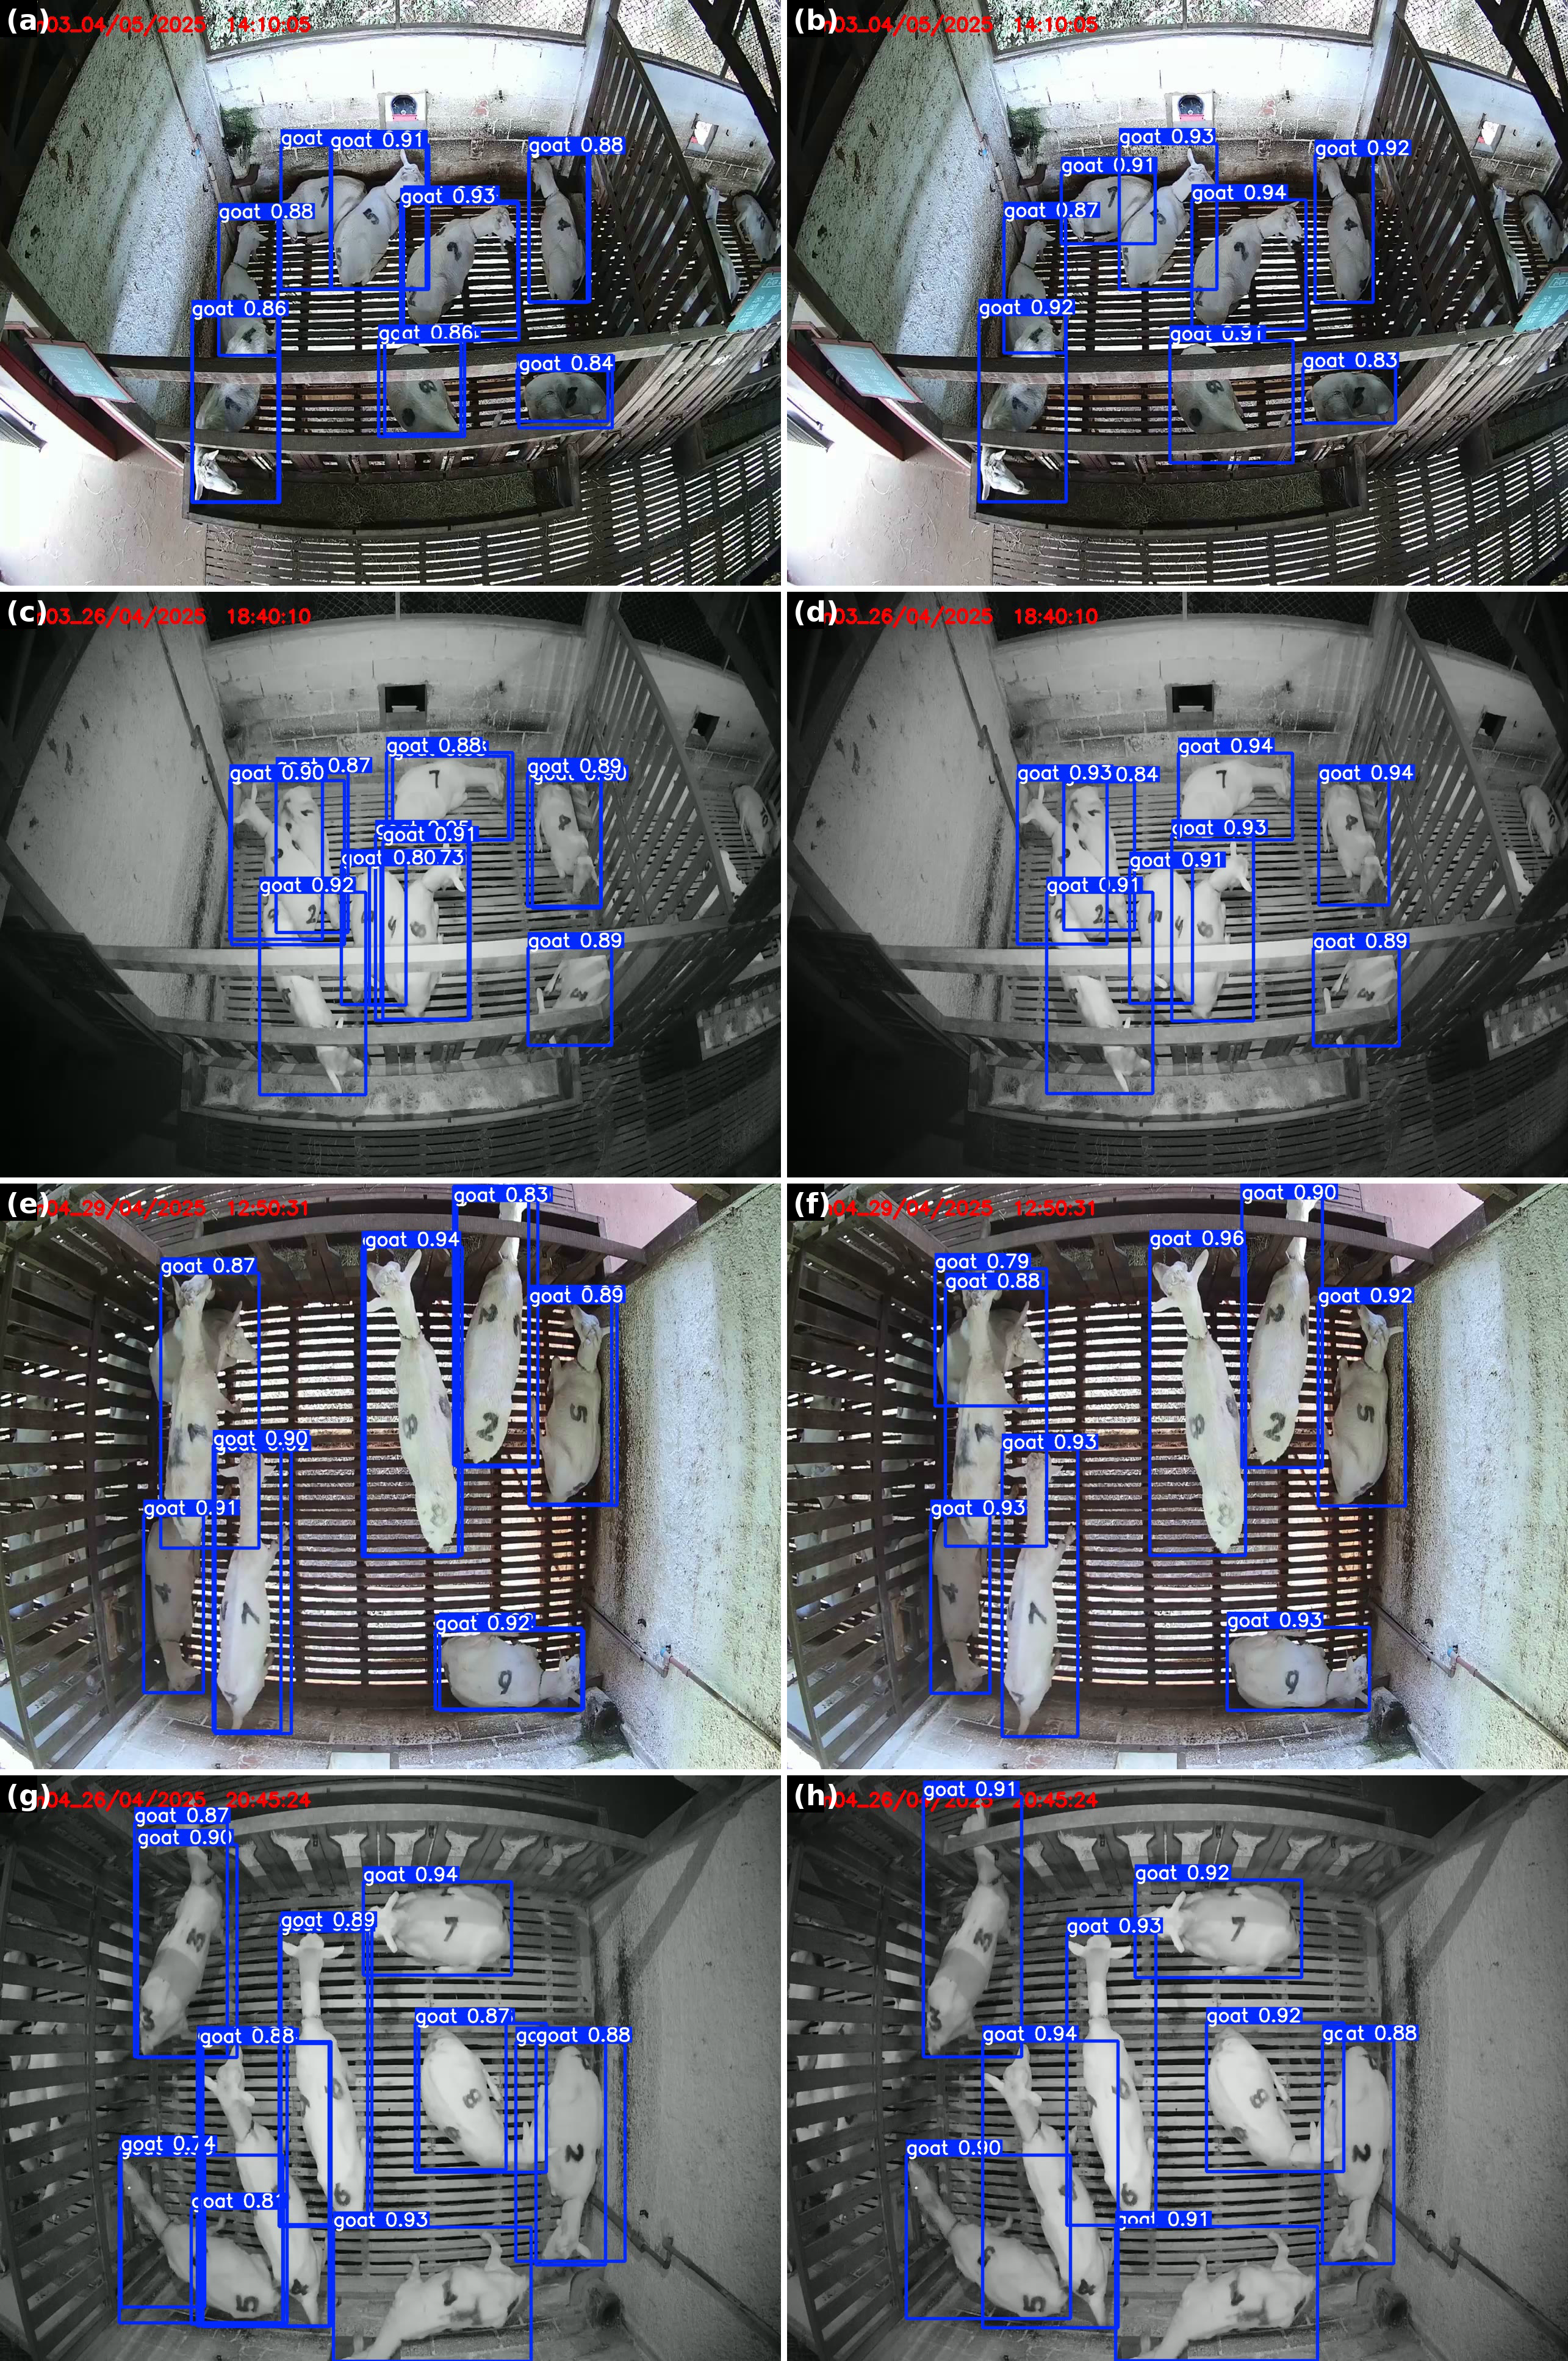
\includegraphics[width=0.72\columnwidth]{figures/comparacao_overall_moe.png}
\\{\bodyfont\small\bfseries Figura 2 -- Baseline (esq.) vs. especialista MoE (dir.) no mesmo quadro:\\ (a-b) Frente Dia, (c-d) Frente Noite, (e-f) Cima Dia, (g-h) Cima Noite}
\end{center}

\vspace{1cm}

% ============================================================================
% CONCLUSÕES
% ============================================================================
{\sectionfont CONCLUSÕES}

{\bodyfont
A arquitetura MoE proposta apresentou desempenho elevado e consistente na detecção de caprinos nos quatro cenários de perspectiva/iluminação avaliados. Embora as métricas agregadas de detecção não demonstrem superioridade da MoE sobre o baseline monolítico, a inspeção qualitativa em vídeo evidencia maior estabilidade da contagem de indivíduos por especialista, além das vantagens estruturais de \textbf{modularidade}, \textbf{isolamento de falhas} e \textbf{explicabilidade} do roteamento.

\textbf{Trabalhos futuros:} rastreamento individualizado dos animais (\textit{multi-object tracking}) para análise comportamental de bem-estar animal; expansão do ecossistema com novos especialistas para cenários adicionais, sem retreinar os demais.
}

\vspace{1cm}

% ============================================================================
% AGRADECIMENTOS
% ============================================================================
{\sectionfont AGRADECIMENTOS}

{\bodyfont
Os autores agradecem à Universidade Federal de Juiz de Fora (UFJF), à Universidade Federal de São João del-Rei (UFSJ) e ao Departamento de Zootecnia da UFSJ pelo suporte no desenvolvimento deste trabalho.
}

\vfill

\end{multicols}

\end{document}
